\chapter{\uppercase{Data-Driven Maps and Consistent Inversion} \label{chapter:04}}

Going off the previous chapter, we may be interested in a different question, and may be in situations where we can collect data easily (or it has already been collected for us).
What are the other types of questions we can ask? Parameter Identification.

We focus on extending the DCI framework to situations where we want to answer a different question.

\
\section{A Generalized Stochastic Map Framework}
%% EDIT THE FOLLOWING BELOW!
Such observable values of $u\lam$ are mathematically modeled by functionals of the solution, denoted $\obs_i: u\lam \to \RR$.
The collection of such functionals into a vector defines a {\em Parameter-to-Observables} (PtO) map, denoted $\obs( u\lam )$ or $\obs\lam\in\RO$ for short.

The observable data is then naturally denoted as $\obs(\pspace)$, and any subsequent transformation of this vector (e.g. averaging, sub-selecting) is captured by the definition of a {\em Quantity of Interest} (QoI) map, denoted $\qoi$.

Since the solution to the model, $u\lam$, depends on $\param$, so do the QoI, and we adopt the notation that $$\qlam := \qoi(\obs(u\lam))$$ to make this dependence on model parameters explicit.

\begin{figure}[ht]
\begin{minipage}{.975\textwidth}
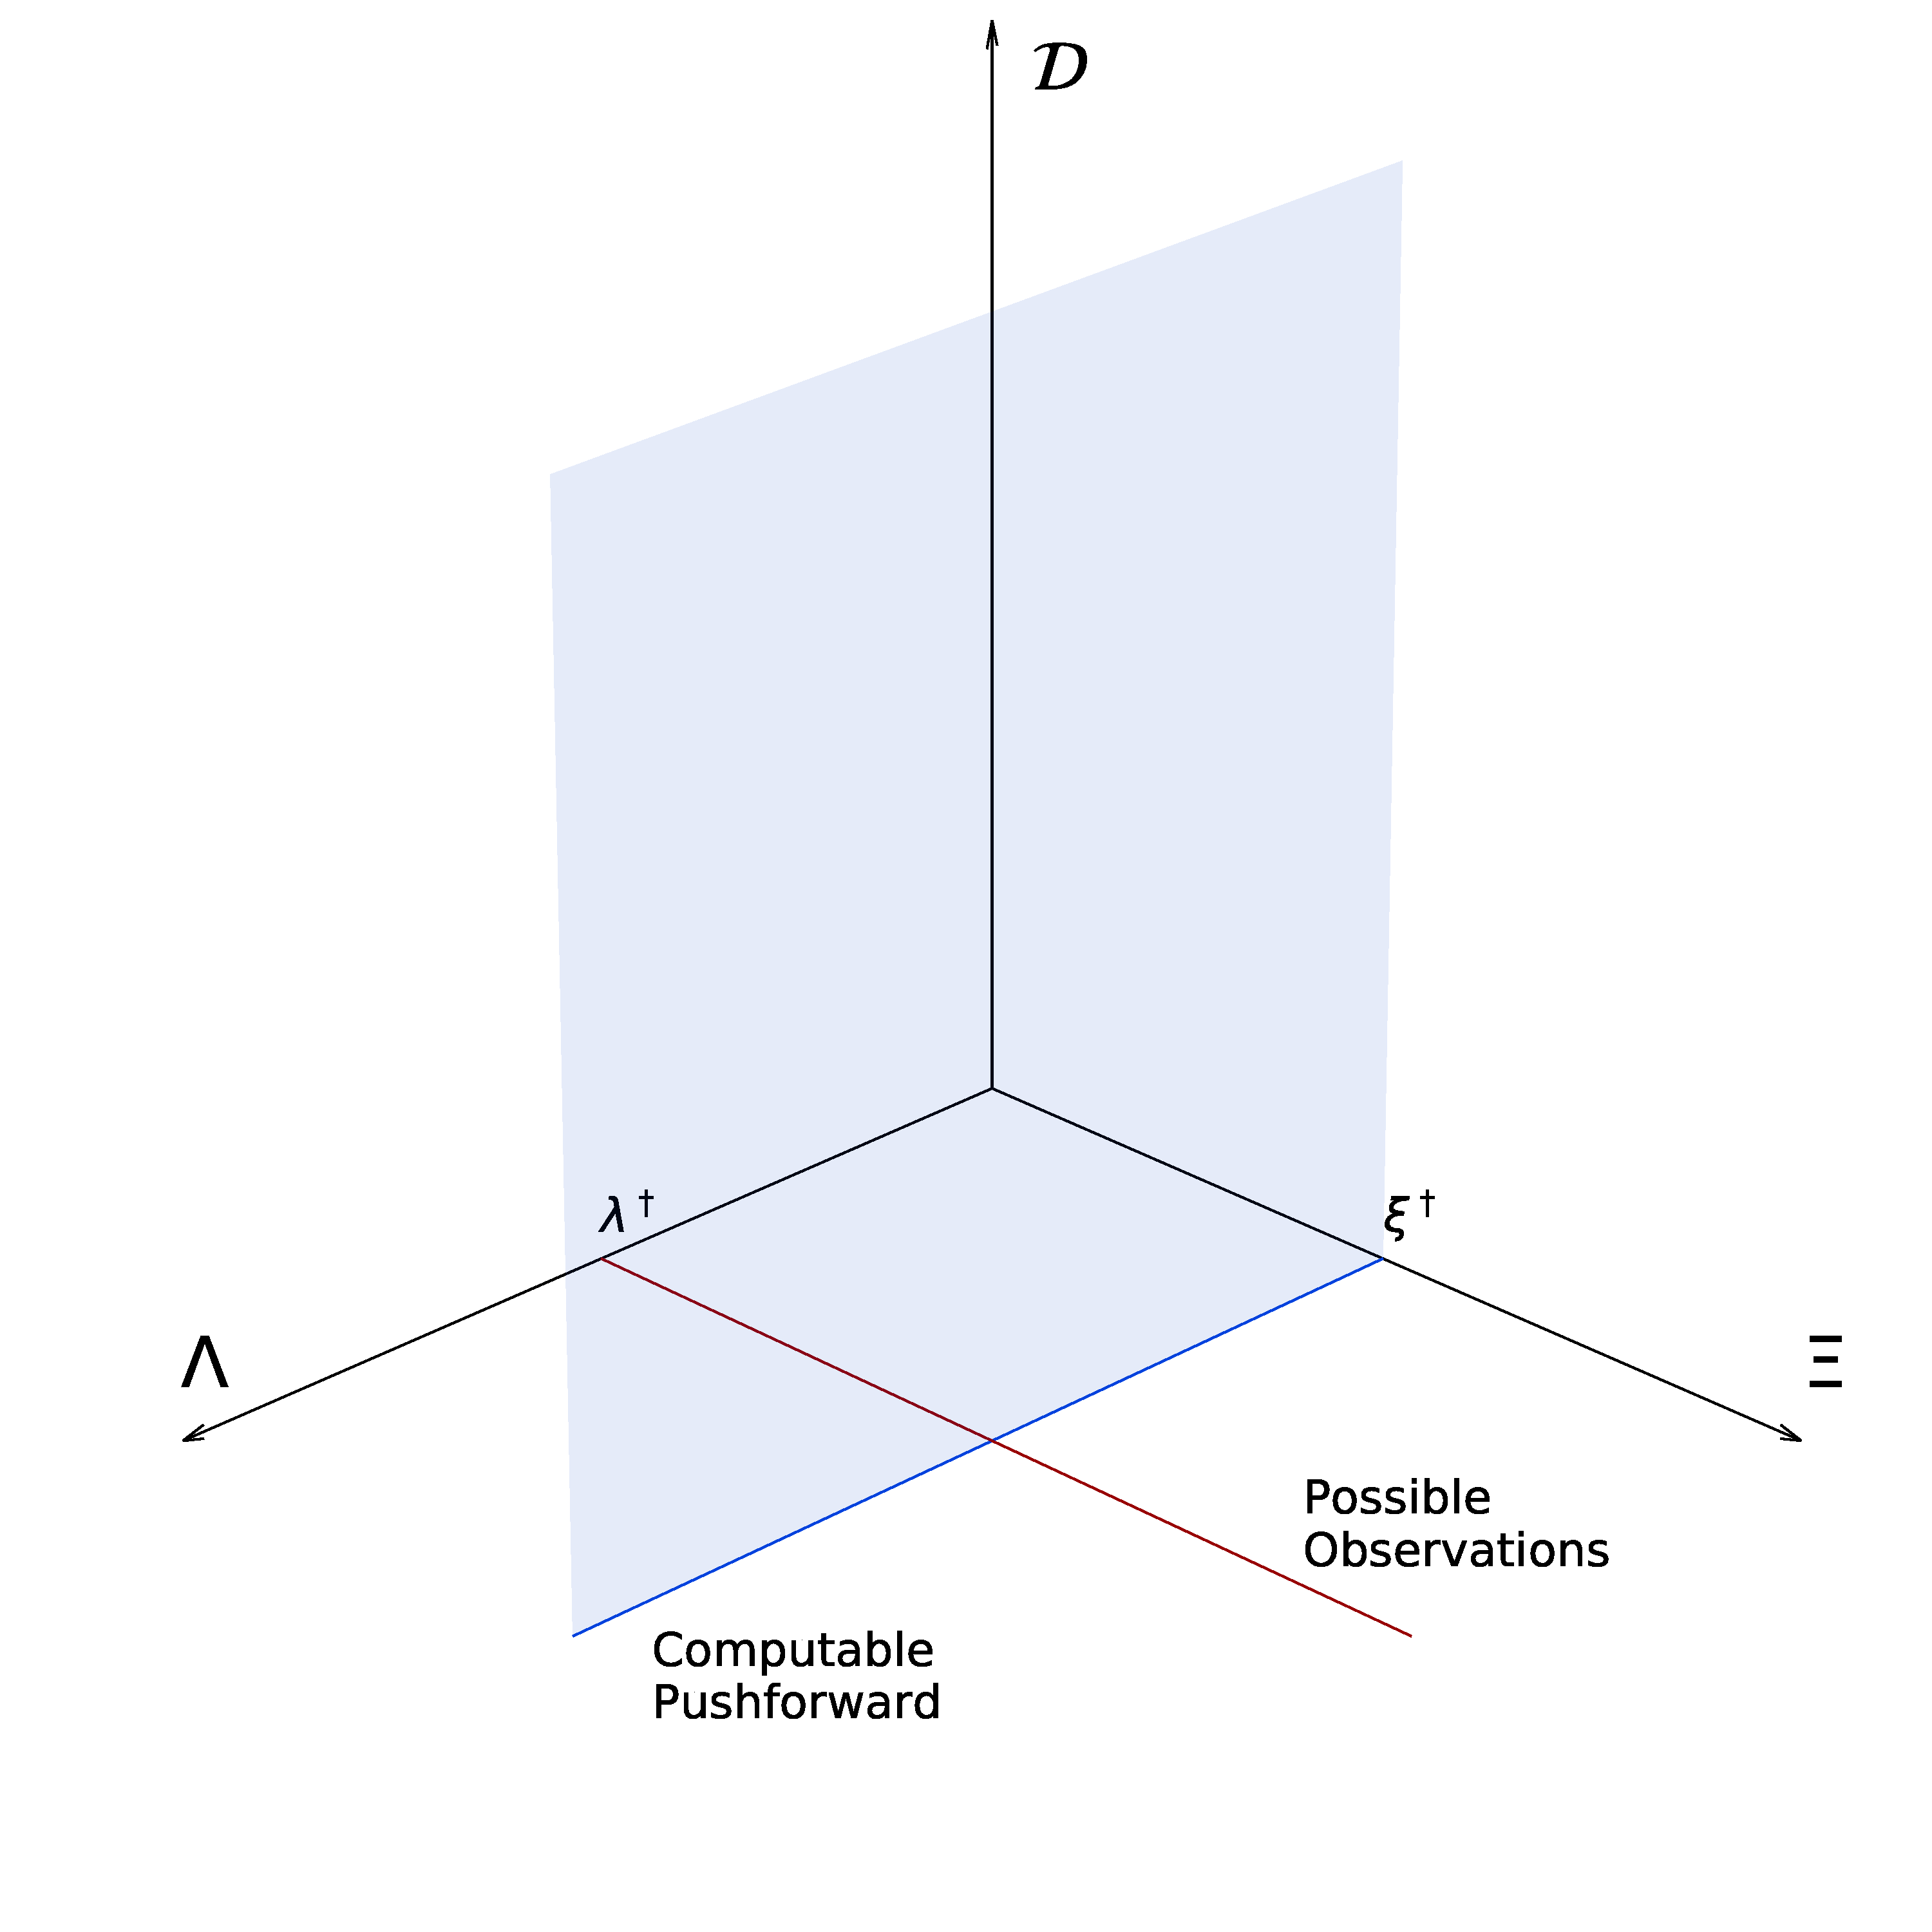
\includegraphics[width=\linewidth]{./images/stochastic_framework.pdf}
\end{minipage}
\caption{
The space of possible observations represents the full range of measurements that could have been collected.
The computable pushforward is a conditional of the full observable space, based on the noise that actually polluted the measurements once they have been taken.
}
\label{fig:stochastic_framework}
\end{figure}
\FloatBarrier

Set stage with the work Troy has been doing lately.

\
\section{Data-Driven Maps}

More material from the paper, including sensitivity analysis with number of data points.

Theory... TK - closed form in 1D


\subsection{Extension to Multiple Quantities of Interest}

This kind of brings us back around to the topic of skewness and OED. Don't get too involved, but do mention it and follow up in the OED discussion in later chapter.

For now, here is basically what needs to be the takeaway:

TK - when you have more than 1 QoI, you can just collapse all the information into one. This doesn't really respect units or differences in information sources, requires minor modification wherein you divide by each variance.

TK - The other option is to iterate between them and converge towards an intersection. What happens when we have error is that the intersection of any pair may be in different places. Less error = less variability in this regard.
Algorithmically, we bounce around in that region, trading off precision (each step loses accuracy in prior directions in favor of increased accuracy of another).


\subsection{Numerical Approximations and Analysis}


TK - If you do not know the variance of your data, then you can approximate it. The theory that comes from this is related to approximate maps converging. good estimates of variance occur at relatively low sample sizes.

\subsection{Descriptions of Error}

\subsection{Examples}

Identity map that is growing.

\
\section{Software Contributions}

Module into BET (started off as CBayes, make footnote or include in appendix) that transforms time-series into QoI and performs data-consistent inversion.
This is implemented as a ``mode'' in BET that can be triggered.
May or may not auto-detect when to use it?

How might ``the user'' interact with these sorts of problems where there is a large matrix of output data?

\
\section{Numerical Results and Analysis}

\subsection{Parameter Estimation and Precision with Time-Series Models}
Take the exponential decay problem and show what happens as we increase the number of data points.

\subsubsection{Fixed-Time}
NOTE: third column of the CSE poster goes here as one example (fixed interval of time).

\subsubsection{Fixed-Frequency}
Next example has fixed measurement frequency.


First, in fixed-time window (say, [1,2]), then at fixed frequency, go up to 100 measurements. Show results.

Show a problem with repeated observations (so, slightly different context, but similar question, and now in a position to compare the measure and density approaches). Use example that was presented at SIAM AN18, except re-formulated as measuring the weight and volume of a liquid.
